\subsection{Attack Goal and Threat Model}
\textbf{Attack goal: Fail both LiDAR and camera perception neural networks in an AV system.}
In this project, we target at evaluating the effectiveness of the MSF-ADV\cite{msf-adv} attack on the synthesized scene.
The attack goal is straight-forward for affecting the safety of autonomous driving: 
fail the AV perception with LiDAR and camera sensors in the target AV, so that it can't detect the obstacle in front of it and collide with it.
This attack also assumes the AV system has a fail-safe mechanism for an emergency brake. 
Even though the system is equipped with an Automatic Emergency Brake(AEB), 
prior works still show that the victim's vehicle can be hit by the cars behind if they fail to brake in time.
Therefore, MSF-ADV is designed for real-world physical attacks with the current industry-level AD systems.

AV systems that use more than 2 perception sensors will usually be equipped with an MSF algorithm,
which is to fuse the information from all of the sensors and then make decisions.
MSF still has the chance to correct the wrong sensor perception as long as there is at least one clean sensor source, which is unattacked.
Since this attack aims at defeating the MSF-based AD perception, it must fail all the sensor perceptions for high attack effectiveness.
Thus MSF needs to attack all visual sensors (i.e., camera and LiDAR) at the same time.

\textbf{Threat Model.} 
MSF-ADV\cite{msf-adv} is designed in a white-box setting. 
It assumes that the attacker knows the MSF algorithm and the corresponding neural network model for each sensor perception in the target AV system.
Many prior works that study physical adversarial attacks towards sensor perception in AV systems also have similar assumptions\cite{adv1, adv2}. 
This assumption is valid as the attacker can reverse engineer the purchased or rent AV perception module to get the algorithm details.
What's more, lots of open-source industry-level AV algorithms can also be the victim, e.g., Baidu Apollo\cite{apollo}, Autoware.AI\cite{autoware}.

Since this attack is closely related to the road condition and background, 
the attacker is also assumed to take camera images and LiDAR data about the target road background to generate the adversarial objects using MSF-ADV.
After getting the adversarial object in the target background, the attacker can 3D print the object and place it at the calculated place.
To make the attack more powerful, the attacker can even fill it with high-density material like granite to make it heavier.
As a result, when the car fails to detect this object and collides with it, the damage might be more severe.
Fig. \ref{fig: noisy} shows the benign object, i.e., a chair, and the malicious chair generated by MSF-ADV\cite{msf-adv}. We can notice that the surface of the malicious chair is more glitchy and it's easy for the vehicle ignores the overall shape and crash into it.

\subsection{Design Challenges}
In the state-of-art work in generating adversarial physical 3D objects,
they all use rendering functions to simulate the sensor outputs and integrate the rendering output with the road background to get the attack-influenced scenarios.
Although many works provide rendering pipelines, we find that simply feeding them with different objects and backgrounds won't meet our requirements due to 4 unique challenges:

\textbf{C1. Need to identify factors in the synthesized scene which might influence the detection accuracy of the neural network.}
To evaluate the authenticity of the synthesized scene, we need to find the factors that might make this scene more realistic or the opposite.
However, these factors are not fully explored in prior work.
When an adversarial object is generated in a previous study, they only consider certain conditions, e.g., specific background, and fixed relative position.
For example, for 3d physical attacks, previous work predominantly considers the relative position between the obstacle and the target vehicle\cite{25}, 
the condition of target road background\cite{msf-adv, lidar1}. 
Although there are many other factors such as the aspect ratio of the background and light conditions, 
they aren't taken into consideration in previous works when synthesizing the scene.
One possible solution is to pick different obstacles and road backgrounds as many as possible.
However, this not only adds up the testing overhead and thus decreases the testing efficiency, 
but also results in redundancy in testing cases, which might influence the trust in the final results.
Thus, it is highly desired to identify some factors that can represent the difference between various synthesized scenes.

\textbf{C2. Physical consistency between the obstacle and the driving background should be maximum guaranteed.} 
To ensure the synthesized scene is generated realistically in the first place, 
prior works are trying to select a physically realizable object such as the drones holding a cardboard with reflective surface\cite{25} and printable traffic cone\cite{msf-adv}.
Since these adversarial objects usually need a lot of optimization iterations to be generated, 
it's impractical to drive the vehicle and put the obstacle in real-life to get real-time adversarial outputs.
Therefore, most prior work will synthesize the impacts of adversarial obstacles from the physical sensor to both image and point cloud outputs, as well as integrate them into the road background.
Despite the consideration of the physical realizability of the object, we also need to model the physical consistency when integrating the object and the background.
For example, no matter where we put the obstacle, it should stand on the road instead of floating in the air or even hitting the ground. 
This means we can't put the obstacle in the background with a random position, instead, the physical model between the obstacle size and relative position should be established.
It should also follow the shadow caused by sunlight. 
For example, the road background is taken when there is light from the east, thus the original object in the background has the shadow facing west.
When the obstacle is put on the road, it's also supposed to have a shadow in the same direction.
Or the neural network may fail to recognize it because of the physical inconsistency.

\textbf{C3. Domain-specific metrics for quantifying the authenticity of the synthesized scene. }
In previous works designing adversarial obstacles, they adopt the optimization-based method,
an optimization loss function is designed to measure the effectiveness of the adversarial object, as well as the stealthiness of the malicious obstacle.
These loss functions are designed based on the confidence value of the object detection neural network, which reflects the probability that the region contains an object\cite{msf-adv}. 
Also, they use metrics to measure the smoothness of the surface of the object.
However, these metrics are designed in a way to make the optimization process more convenient, and faster.
Our preliminary experiments show that even after the optimization, it's still possible for the neural network to detect the obstacle.
Therefore, we have to come up with new metrics to measure the performance of the object detection neural network and the adversarial attacks.
Meanwhile, previous works use different metrics to measure whether their adversarial obstacle achieves the goal and lack a unified standard, 
which makes it difficult to provide fair and reasonable metrics. 

\textbf{C4. Develop an automated pipeline for generating different synthesized scenes. }
After obtaining the factors that influence the authenticity of the synthesized scenes, corresponding value ranges should be determined.
Usually, the prior works only consider limited factors with certain value ranges, 
the rendering pipeline they're using may not be suitable for comprehensive testing.
It's also unrealistic to manually choose the combinations among factors as this takes a lot of effort.
Automated pipelines generating different testing scenarios should be developed.
Meanwhile, since different synthesized scenes are generated to measure its authenticity through evaluating the neural network's performance in benign and malicious cases,
this pipeline should also be equipped with neural network model inference and automatically compute the evaluation metrics along the way.
Having this automated pipeline can help us to do a large-scale analysis on how realistic these synthesized scenes are.

\begin{figure}
	\centering
	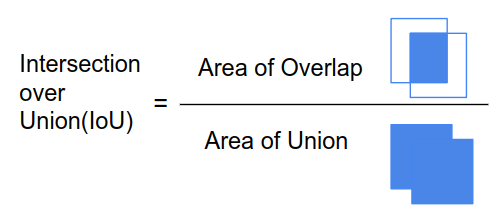
\includegraphics[width=0.5\linewidth]{figure/iou.png}
	\caption{Intersection over Union(IoU)}
	\label{fig:iou}
\end{figure}

\begin{figure*}
	\centering
	\begin{subfigure}{0.5\textwidth}
		\centering
		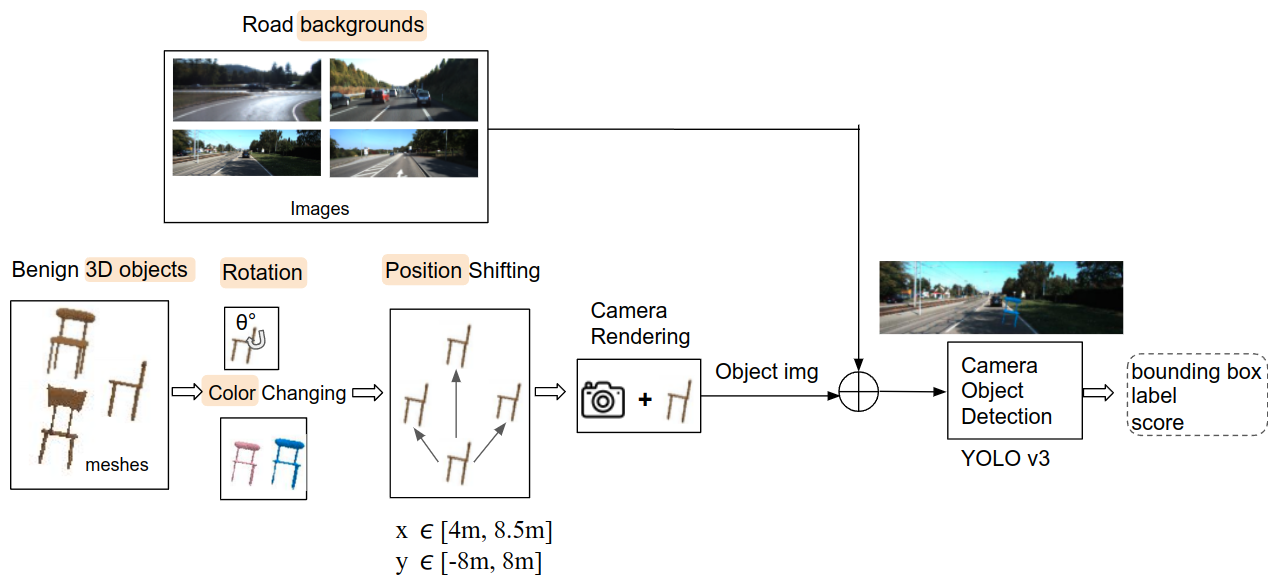
\includegraphics[width=0.7\linewidth]{figure/test-pipeline.png}
		\caption{Overview of the automated test suite pipeline for benign synthesized scenes.}
		\label{fig:test-pipe}
	\end{subfigure}%
	\begin{subfigure}{0.5\textwidth}
		\centering
		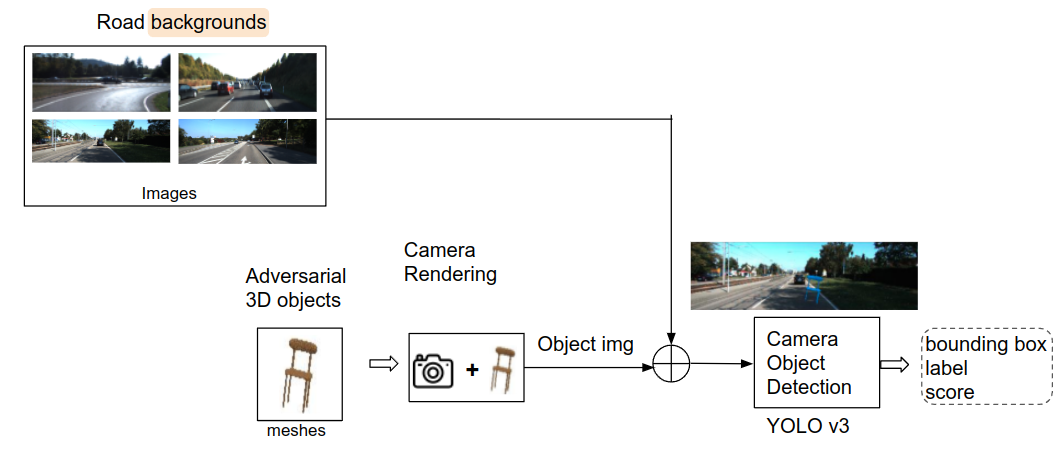
\includegraphics[width=0.7\linewidth]{figure/test-attack.png}
		\caption{Overview of the automated test suite for adversarial synthesized scenes.}
		\label{fig:test-att}
	\end{subfigure}
	\caption{Detection rate and confidence rate for benign objects}
	\label{fig:pipe}
\end{figure*}

%\begin{figure}
%	\centering
%	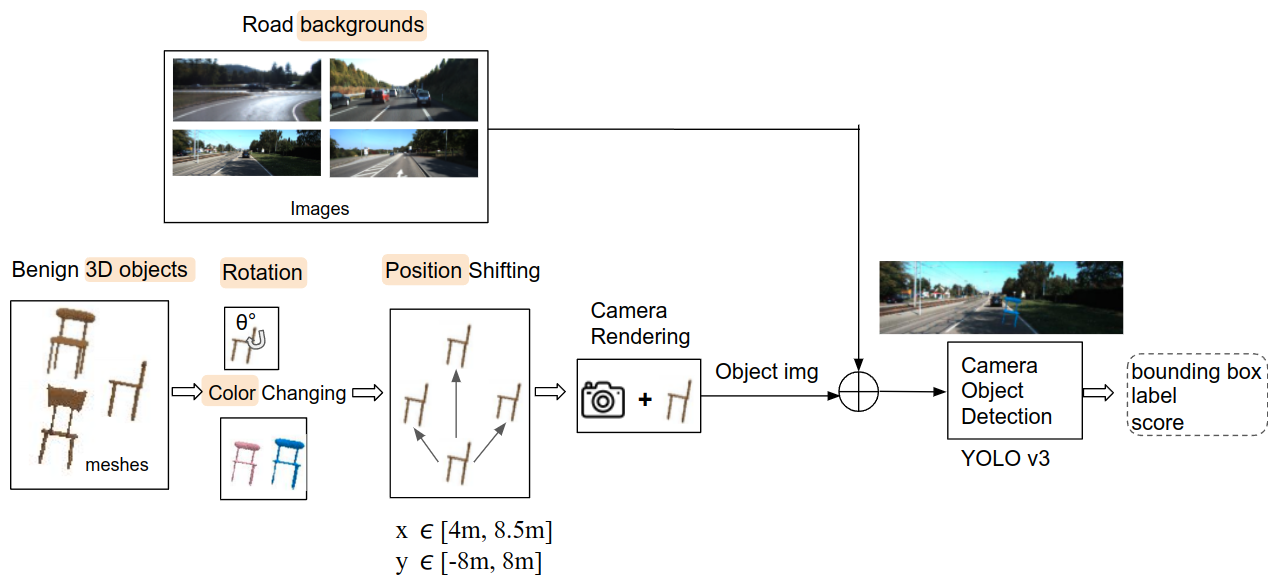
\includegraphics[width=1\linewidth]{figure/test-pipeline.png}
%	\caption{Overview of the automated test suite pipeline for benign synthesized scenes.}
%	\label{fig:test-pipe}
%\end{figure}


%\begin{figure}
%	\centering
%	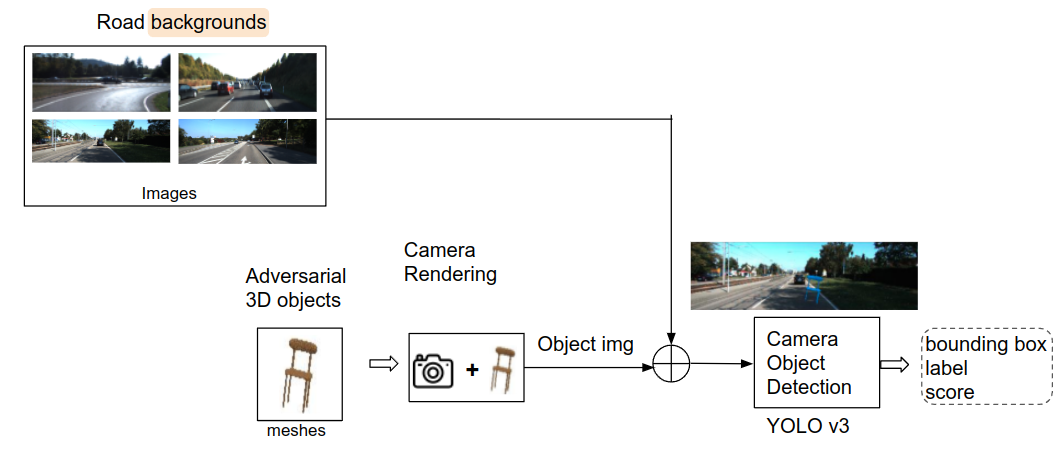
\includegraphics[width=1\linewidth]{figure/test-attack.png}
%	\caption{Overview of the automated test suite for adversarial synthesized scenes.}
%	\label{fig:test-att}
%\end{figure}

% -----------
\begin{figure}
	\centering
	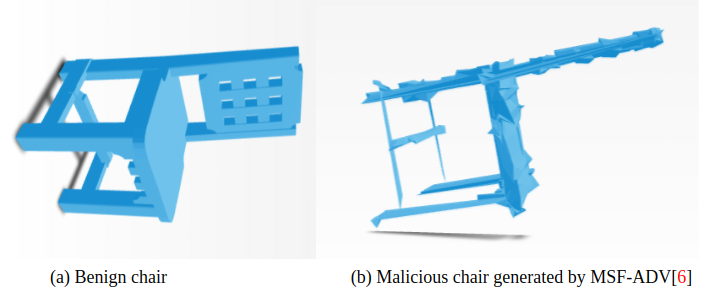
\includegraphics[width=1\linewidth]{figure/benign&ma.png}
	\caption{Benign chair and the malicious version}
	\label{fig:noisy}
\end{figure}
% -----------------
\begin{figure*}
	\centering
	\begin{subfigure}{0.5\textwidth}
		\centering
		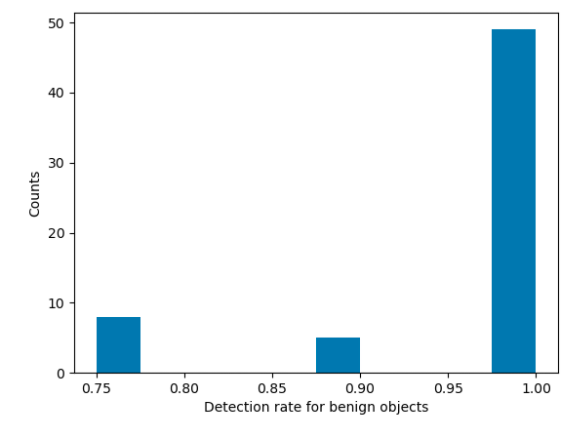
\includegraphics[width=0.7\linewidth]{figure/detection-rate-b.png}
		\caption{Detection rate for benign objects}
		\label{fig:det-b}
	\end{subfigure}%
	\begin{subfigure}{0.5\textwidth}
		\centering
		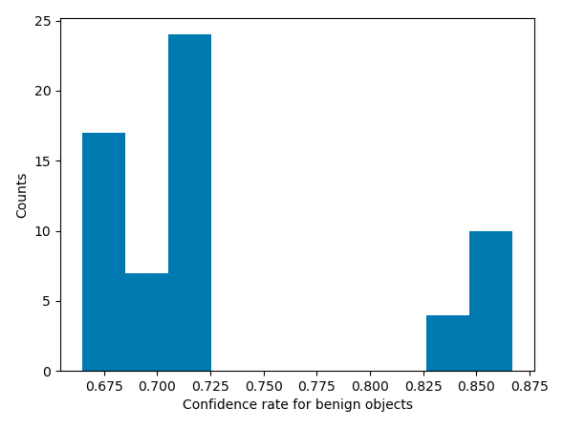
\includegraphics[width=0.7\linewidth]{figure/conf-rate-b.png}
		\caption{Confidence rate for benign objects}
		\label{fig:conf-b}
	\end{subfigure}
	\caption{Detection rate and confidence rate for benign objects}
	\label{fig:swat}
\end{figure*}
